Nowadays, the need for the visualization of software quality metrics has been rapidly increased. Software metrics help developers and companies to check and analyze information about the performance, quality of code and cost of software data. it helps to find out and fix errors in the early stages of development.

In this chapter will be described some tools for visualization of software quality metrics and tool for code analysis.

\section{Open Source tool "METRIX"}

This tool can compute different software quality metrics. METRIX is able to evaluate software written in C and ADA languages and many metrics can be considered for software evaluation (the different metrics will be described in detail in the next section ~\cite{metrix}. 

The user can use different types of diagrams for metrics visualization: histograms, scatter plots and line charts. 
This tool allows to use two not common classes of diagrams: 

\begin{itemize}
	\item The first is Kiviat diagrams, also known as the radar plots.
	\item The second is the city map diagram.
\end{itemize}

One specific feature of METRIX is to use those two types of visualization for constructing signature and cartography of source codes ~\cite{metrix}.
 
\textbf{Kiviat diagrams}
The Kiviat diagram uses polar coordinates for visualization. The value which user wants to represent associated with the distance between the point and the origin. The angle between two points does not change because it is constant. This constant is calculated to uniformly distribute the different points. Linked together metric points make a plain polygon, which forms the data specifics of represented values. This type of diagram can be used only for visualization of more than three values of calculated metric. All values must be strictly positive. The user can merge data in one diagram. Also, this tool allows drawing the diagram for one or several metrics together. 

In Figure \ref{fig:metrix} shows an example of two Kiviat diagrams. These diagrams represent different metric values for two functions. 

\begin{figure}[ht]
	\centering
	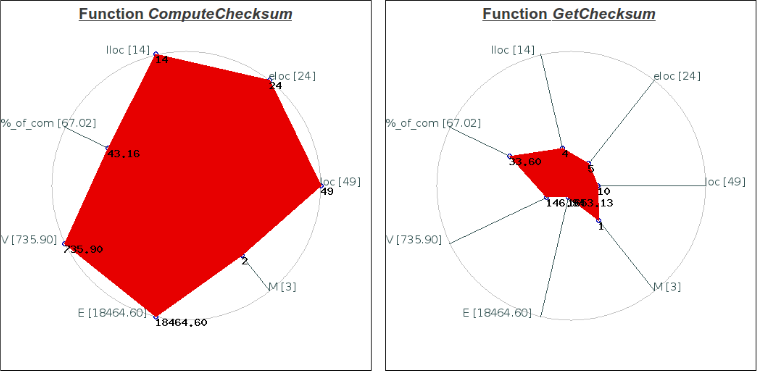
\includegraphics[height=70mm]{figures/metrix.png}
	\caption{An example of Kiviat diagrams.}
	\label{fig:metrix}
\end{figure}

\textbf{City map diagrams}
Usually this type of diagrams used for representing cities with buildings in three dimensions. City map diagrams also suit for visualization of software metrics of the project with a large number of source files, functions and variables. Source code metrics are represented by rectangles by using the treemap diagram. Some authors used variants of this class of visualization diagrams to represent  values with esthetic considerations. City map diagrams are indeed multi-parameters diagrams: each “building” is associated with an n-tuple of numeric values ~\cite{metrix}.  

This tool also has a graphical user interface with a single Window containing three tabs: “Calc”, “Csv” and “Plots”.

In the first "Calc" tab user chose source files for evaluation and also chose metrics which neede to be measured.It allows to users to use  hand-start scripts with a prompt. The open source aspect of the tool allows users to repeat the measuring scripts manually or to integrate them into other software.

In the second “Csv” tab user can find a list of numeric values and chose which values will be used for function or for the file. There is an option for exporting calculated values to a spreadsheet application for drawing graphs, like scatter plots, line plots, etc.

In the third “Plots” tab the user can build the city map diagrams for the source code. The user can change the settings of the tool like the modification of placement of the buildings in the city map or make the data colored, etc.

This tool supports making a report in the form of a LaTeX file where each function and each file make a section of this report. User can use PDF file for analisis. This report includes all the values measured on the project. Each file produces three views of the associated city map diagram, as well as different Kiviat diagrams for the different metrics measured on the functions of the file ~\cite{metrix}. 

\section{Sextant}

Sextant is a Java source-code analysis tool under development at the University of Nebraska at Omaha (UNO) ~\cite{sextant}. This software is a complex extension of the TL system (a general-purpose program transformation system) created particularly for the Java programming language domain.

The main design goal of Sextant is providing a tool facilitating specification and visualization of custom analysis rules, which can be domain-specific or moreover application specific analysis rules.

Analysis rules of Sextant are based on information fetched from different software models. There are two main models of central importance. The first model is a syntactic model. It is the source code parse tree. Parse trees conform to compilation units which represented by Java files and are generated with use of GLR parser technology provided by the TL system. Parse trees are well-fitted for analyzing and manipulating through standard primitives provided by program transformation systems, for example, by matching and generic traversal.

The second model is a compound attributed graph (CAG). It is a semantic model which captures subtype, structural, and reference dependencies among the constructors, methods, fields, packages and types. The CAG also links an attribute list with every node and edge.

CAG information is accessible to Sextant’s transformation-based analysis rules via two mechanisms. The first mechanism is a positional system which organizes a relation between contexts within the CAG and corresponding parse (sub)trees. This relation makes possible correctly resolving references to constructors, methods, types, fields, and local variables, during the process of generic traversals which are the key enabling mechanism in program transformation systems.

The second mechanism is a library of semantic queries. These queries can be accessed even in the middle of transformation course. Functionality which provided by this library contains things like:
\begin{itemize}
	\item Reference resolving.
	\item Reference type determining.
	\item Determining declaration shadowing or overriding.
	\item Determining whether one type is a subtype of another.
\end{itemize}
 
Sextant stores table and set types for information collecting with relation to analysis rules. These constructs can be used for storing information related to a custom metrics wide variety.

Sextant is open-ended with respect to the definition of metrics – any source-code analysis rule can be interpreted as a metric, be they PMD-style rules focusing on violations of coding conventions or rules such as those specified by FindBugs that are more semantic in nature \cite{sextant}.

Sextant can do software models generation. These models can be visualized using other tools such as GraphViz, Cytoscape and TreeMap. Sextant can produce the CAG of the code base in a JavaScript object notation format (JSON). This JSON file can be loaded into Cytoscape, an open source platform which provides extensive and sophisticated capabilities for large complex networks visualization, for example, graph structures. The same way, metrics derived from sets and tables can be produced in CSV format and viewed with use of TreeMap. Parse trees can be output as dot-files and later viewed with use of GraphViz.

The view in Figure \ref{fig:1} shows an example of represents a coloring of dependencies on the unsupported features. Nodes colored orange have indirect dependencies on unsupported features while purple nodes have direct dependencies on unsupported features.

\begin{figure}[ht]
	\centering
	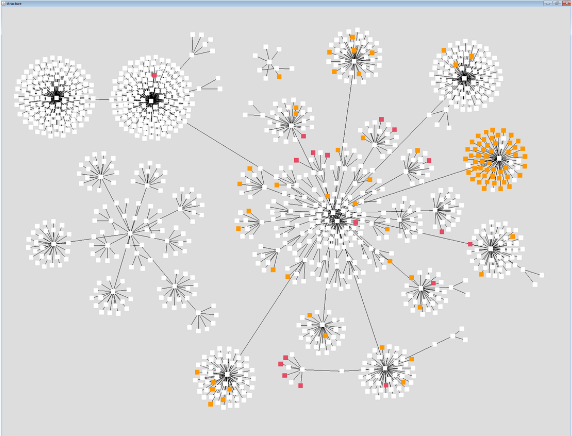
\includegraphics[height=70mm]{figures/1.png}
	\caption{An example of using Sextant tool.}
	\label{fig:1}
\end{figure}

\section{NDepend}

NDepend is a static analysis tool for .NET managed code. The tool can measure a large number of code metrics, allowing to visualize dependencies using directed graphs and dependency matrix.  

NDepend computes many size-related metrics: number of lines of code, number of assemblies, number of types, number of methods, etc. For measuring complexity, NDepend uses Cyclomatic Complexity. This metric calculates the complexity of a method or a type by calculating how many branching points it contains in the code.

NDepend has two metrics for cohesion. Relational Cohesion is an assembly level metric that calculates the average number of internal relationships for each type. Lack of Cohesion Of Methods (LCOM) measures a type cohesiveness. A type is maximally cohesive if every method use all instance fields.

NDepend has a tool for visualization called a Treemap. Also, NDepend has a dashboard for quick visualization of all application metrics. It's shown in Figure \ref{fig:dash}. The dashboard is available as the extension for Visual Studio. The dashboard shows the diff since baseline for every metric. It also displays if the metric value becomes better (in green) or worse (in red). 

\begin{figure}[ht]
	\centering
	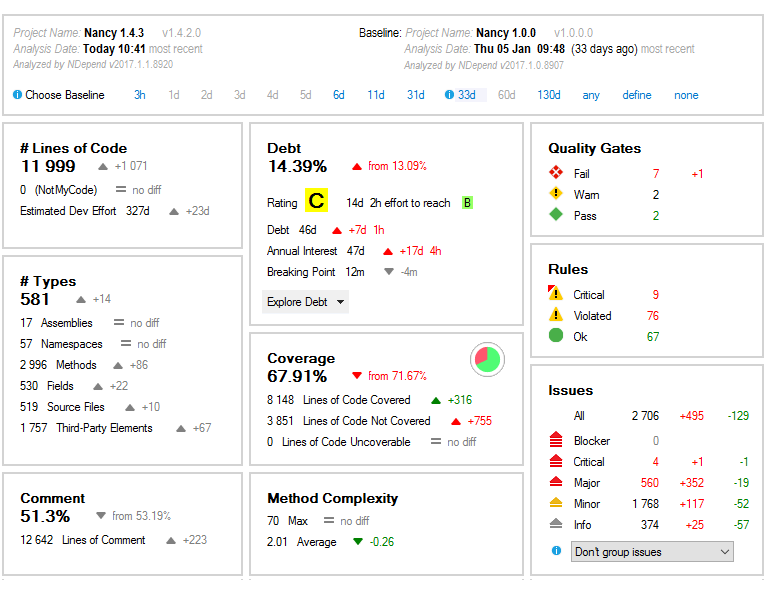
\includegraphics[height=70mm]{figures/dash.png}
	\caption{An example of using the dashboard.}
	\label{fig:dash}
\end{figure}

The Figure \ref{fig:tree} shows metric visualization using the colored treemap.

\begin{figure}[ht]
	\centering
	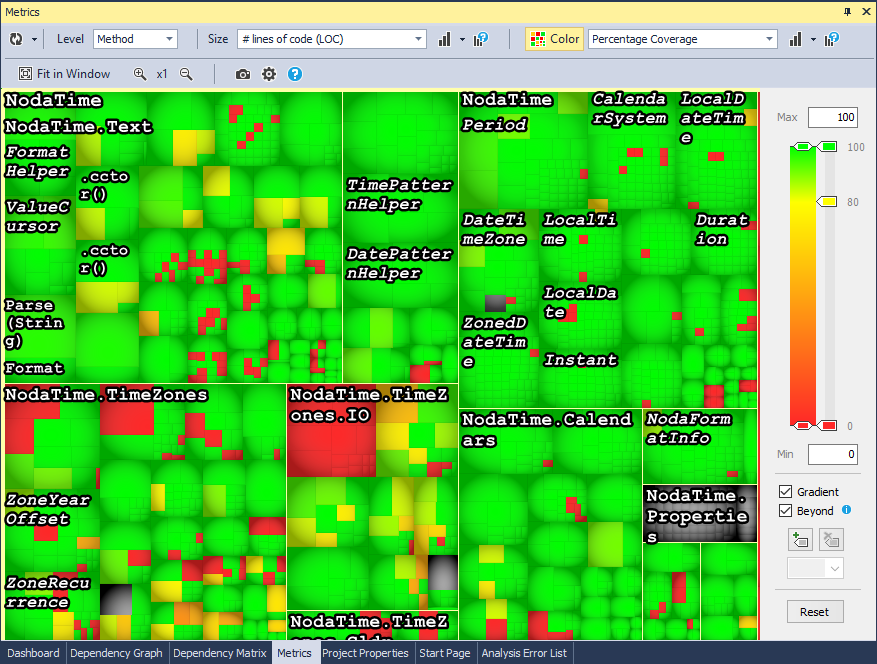
\includegraphics[height=70mm]{figures/tree.png}
	\caption{An example of using the colored treemap.}
	\label{fig:tree}
\end{figure}

The tree structure used in NDepend treemap is the usual code hierarchy: 

\begin{itemize}
	\item .NET assemblies contain namespaces.
	\item Namespaces contain types.
	\item Types contain methods and fields.
\end{itemize}

\section{PVS-Studio}

PVS-Studio is a tool for detecting bugs and security weaknesses in the source code of programs, written in C, C++, and C\#. It works in Windows, Linux, and macOS environment ~\cite{pvs}. The user can use online reference manual concerning all the diagnostics methods available in the program and  on the website.

This tool executes static code analysis. The generated report helps developers in debugging. PVS-Studio has large number of methods for checking. These methods help to find typing and copy-paste mistakes. The main value of static analysis is in its regular use so that errors are identified and fixed at the earliest stages ~\cite{pvs}. 				

PVS-Studio can work on a Linux environment on Windows. It can be run from the command or can be integrated into Visual Studio development environment. The results of the analysis are presented in the HTML document which allows full navigation through the source code. The Figure \ref{fig:pvs} shows an example of an HTML-report.

\begin{figure}[ht]
	\centering
	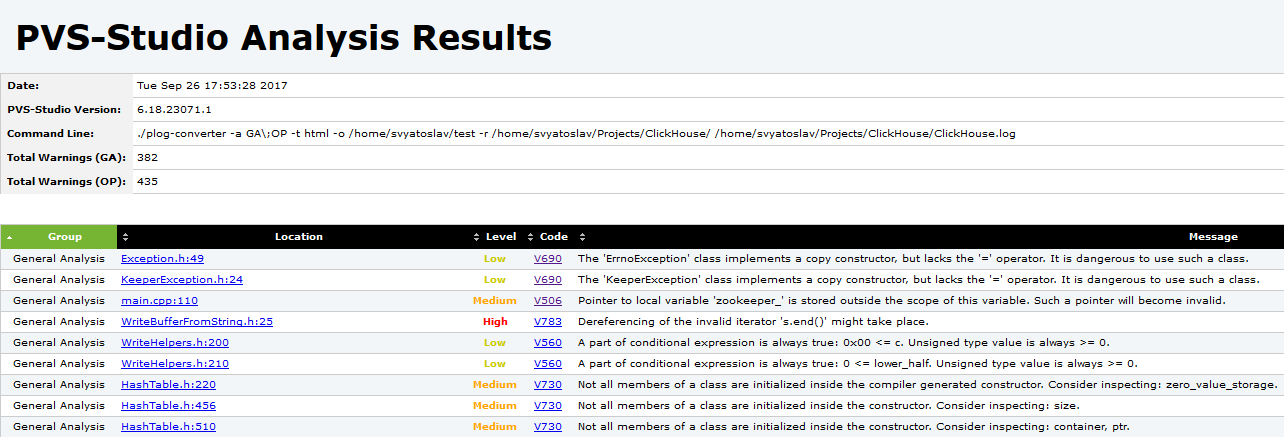
\includegraphics[height=53mm]{figures/pvs.png}
	\caption{Main page of an HTML-report.}
	\label{fig:pvs}
\end{figure}

It is possible to not include files from the analysis by name, folder or mask; to run the analysis on the files modified during the last N days ~\cite{pvs}. PVS-Studio has an integration with open source platform SonarQube. This platform was designed for uninterrupted analysis and evaluation of the quality of code.